

\section{\trAffineScheme{}的\trUnderlyingSet}

对任一\trRing{} $A$，我们将定义一个叫做 $\Spec A$ 的东西：$A$ 的\textbf{\trSpectrum}（spectrum）。本节先把它定义为一个\trSet，但很快我们就会赋予它一个\trTopology，稍后再在其上定义一个环层（即\trStructureSheaf）。这样的对象称为\textbf{\trAffineScheme}（affine scheme）。日后，$\Spec A$ 将指集合连同拓扑以及一个函数层这整个整体。不过眼下既然绝无混淆之虞，$\Spec A$ 就只指那个集合。

\textbf{3.2.1.}\quad $\Spec A$ 这个集合，就是 $A$ 的全部\trPrimeIdeal{}所成的集合。$A$ 的\trPrimeIdeal{} $\mathfrak{p}$，当把它看作 $\Spec A$ 的元素时，将记作 $[\mathfrak{p}]$，以免混淆。$A$ 的元素 $a$ 将称为 $\Spec A$ 上的\textbf{函数}（functions on $\Spec A$），其在点 $[\mathfrak{p}]$ 处的\textbf{值}（value）为 $a\pmod{\mathfrak{p}}$。\emph{这很怪异：一个函数可以在不同的点上于不同的环中取值——$\Spec\mathbb{Z}$ 上的函数 $5$ 在 $[(2)]$ 处取值 $1\pmod{2}$，而在 $[(3)]$ 处取值 $2\pmod{3}$。}

「\trRing{}的一个元素 $a$ 落在\trPrimeIdeal{} $\mathfrak{p}$ 中」翻译过来就是「函数 $a$ 在点 $[\mathfrak{p}]$ 处取值为 $0$」，或者说「函数 $a$ 在点 $[\mathfrak{p}]$ 处消失」，这几个说法我们将不加区分地混用。注意：把两个函数相加（或相乘），就是把它们在所有点上的值相加（或相乘）；这是「$A\to A/\mathfrak{p}$ 是\trRingMorphism」这一事实的翻译。这些翻译很重要——务必要对它们运用自如！它们应当成为你的第二天性。

若 $A$ 在一个基域（或基环）上由元素 $x_1,\dots,x_r$ 生成，则 $x_1,\dots,x_r$ 常被称为\textbf{\trCoordinate}（coordinates），因为日后我们将能借助 \S3.2.10 的想法，把它们重新解释为「$r$ 维空间上的坐标」的限制；精确的版本见练习~7.2.F。

\textbf{3.2.2.\ 代数与几何之间一部宏大词典的开端。}\quad 我们正在着手编纂一部宏大词典的开篇；见 \S3.7.2 的第一部分。到了某个时刻你会有这样的感觉：我们正在缓缓破译一块永恒的罗塞塔石碑，只是碑上的刻文令我们辨认起来颇为吃力。

\textbf{3.2.3.\ 未来的一瞥。}\quad 在 \S4.1.3 中：我们将把 $\Spec A$ 上的函数解释为「\trStructureSheaf」的\trGlobalSections，也就是说，按 \S2.2.13 的意义把它们解释为\trRingedSpace{}上的函数。我们重申 \S2.2.13 的一句警示：我们称为「函数」的东西，别人也许会称作「正则函数」。而我们日后将定义「有理函数」（\S6.6.36），它们并不严格是这种意义下的函数，而是「部分有定义的函数」的一种特殊类型。

「函数的值」这一观念日后将被解释为函数在一个特定的\trLocallyRingedSpace{}上的取值；见定义~4.3.7。

\textbf{3.2.4.}\quad 我们现在给出一些例子。

\textbf{例~1（\trComplex\trAffineLine）：}$\mathbb{A}^1_{\mathbb{C}}:=\Spec\mathbb{C}[x]$。我们来求出 $\mathbb{C}[x]$ 的\trPrimeIdeal。由于 $\mathbb{C}[x]$ 是\trIntegralDomain，$0$ 是素的。此外，对任意 $a\in\mathbb{C}$，$(x-a)$ 也是素的；它甚至是\trMaximalIdeal，因为对这个理想取商得到一个\trField：
\[
0\longrightarrow (x-a)\longrightarrow \mathbb{C}[x]\xrightarrow{\;f\mapsto f(a)\;}\mathbb{C}\longrightarrow 0.
\]
（这条\trExactSequence{}也许会让你想起流形那个动机性例子中的 \eqref{eq:maximal-ideal-sequence}。）

现在我们证明没有别的\trPrimeIdeal{}了。我们用到的事实是：$\mathbb{C}[x]$ 有\trDivisionAlgorithm，并且是\trUFD。设 $\mathfrak{p}$ 是一个\trPrimeIdeal。若 $\mathfrak{p}\neq(0)$，则取 $f(x)\in\mathfrak{p}$ 为次数最小的非零元素。它不是常数，因为\trPrimeIdeal{}不能容纳 $1$。若 $f(x)$ 不是一次的，则可分解 $f(x)=g(x)h(x)$，其中 $g(x)$ 与 $h(x)$ 的次数都是正的。（这里我们用到 $\mathbb{C}$ 是\trAlgClosedField{}这一事实。）于是 $g(x)\in\mathfrak{p}$ 或 $h(x)\in\mathfrak{p}$，与 $f$ 的次数的最小性矛盾。故 $\mathfrak{p}$ 中有一次元素 $x-a$。这时我断言 $\mathfrak{p}=(x-a)$。设 $f(x)\in\mathfrak{p}$。\trDivisionAlgorithm{}将给出 $f(x)=g(x)(x-a)+m$，其中 $m\in\mathbb{C}$。于是 $m=f(x)-g(x)(x-a)\in\mathfrak{p}$。若 $m\neq0$，则 $1\in\mathfrak{p}$，矛盾。

这样一来，我们能够、也应当（而且必须！）为 $\mathbb{A}^1_{\mathbb{C}}=\Spec\mathbb{C}[x]$ 画一幅图（见图~\ref{fig:a1c-picture}）。这只是\trn{Sophie Germain}{苏菲·热尔曼}的一个观点的第一个例证 [Ge]：「代数不过是写出来的几何；几何不过是画出来的代数。」（原句为法语：「L'algèbre n'est qu'une géométrie écrite; la géométrie n'est qu'un algèbre figurée.」）

每个复数各有一个「传统的点」，此外还多出一个（「附赠」）点 $[(0)]$。我们大体上可以把 $\mathbb{A}^1_{\mathbb{C}}$ 设想为 $\mathbb{C}$：点 $[(x-a)]$，我们自然会把它与 $a\in\mathbb{C}$ 联系起来。那么点 $[(0)]$ 该画在哪里？看待它的最好方式颇有几分禅意\footnote{译注：原文作「somewhat zen」。}。它在复直线的某处，却又不在任何特定的地方。由于 $(0)$ 含于所有这些素理想之中，我们将以某种方式把它与这条穿过所有其余点的直线联系起来。这个新点 $[(0)]$ 称为这条直线的\textbf{\trGenericPoint}（generic point）。（我们将在 \S3.6 中正式定义「一般点」。）它「一般地」在这条直线上，但除此之外你便再无法把它钉得更为确切；它并不在这条直线上的任何特定位置。（这么说也有点误导——我们将在容易的练习~3.6.N 中看到，它「贴近」每一个点。所以它贴近一切，却又没有确切的位置。）既然没有更好的地方可放，我们便把它画在很靠右边之处。你会注意到，我们把 $\mathbb{A}^1_{\mathbb{C}}$ 画成一（实）维的样子（尽管我们把它画成 $\mathbb{C}$ 的一个增强版）；这是为了日后提醒自己：这将是一个一维空间，其维数是在代数（或复几何）的意义下定义的。（维数将在第 12 章定义。）

\begin{figure}[htbp]
\centering
\begin{tikzpicture}[scale=0.92]
  \node[align=right] at (-2.3,0.1) {代数\\[-2pt]视角};
  \node[align=right] at (-2.3,-1.6) {几何\\[-2pt]视角};
  \node (a1) at (0,0) {$(x)$};
  \node (a2) at (1.7,0) {$(x-1)$};
  \node (a3) at (3.55,0) {$(x-a)$};
  \node at (5.15,0) {$\subset\ \mathbb{C}[x]$};
  \node (a4) at (8.0,0) {$(0)$};
  \draw[thick] \vkbracedown{-0.55}{4.35}{0.52}{0.15}{0.13};
  \node at (1.9,0.95) {$\mathbb{C}[x]$ 的\trMaximalIdeal};
  \draw[thick] \vkbracedown{-0.55}{8.55}{1.18}{0.15}{0.13};
  \node at (4.0,1.68) {$\mathbb{C}[x]$ 的\trPrimeIdeal};
  \draw[thick] (-0.9,-1.7) -- (8.9,-1.7);
  \fill (0,-1.7) circle (1.7pt);
  \node at (0,-2.05) {$0$};
  \node at (1.7,-2.05) {$1$};
  \node at (3.55,-2.05) {$a\in\mathbb{C}$};
  \node at (6.0,-1.7) {$\cdots$};
  \fill (8.0,-1.7) circle (1.7pt);
  \node at (8.0,-2.05) {$???$};
  \node at (0,-2.6) {$=[(x)]$};
  \node at (1.7,-2.6) {$=[(x-1)]$};
  \node at (3.55,-2.6) {$=[(x-a)]$};
  \node at (8.0,-2.6) {$=[(0)]$};
  \draw[thick] \vkbraceup{-0.5}{4.55}{-3.18}{0.15}{0.13};
  \node at (2.0,-3.62) {$\mathbb{C}$ 的点};
  \draw[thick] \vkbraceup{-0.5}{8.55}{-3.92}{0.15}{0.13};
  \node at (4.0,-4.36) {$\mathbb{A}^1_{\mathbb{C}}$ 的点};
\end{tikzpicture}
\caption{$\mathbb{A}^1_{\mathbb{C}}=\Spec\mathbb{C}[x]$ 的一幅图。（依原书手绘图重绘。）}\label{fig:a1c-picture}
\end{figure}

为了让你对这个空间有些感觉，我们给出若干眼下尚未定义、但富有暗示性的陈述。$\mathbb{A}^1_{\mathbb{C}}$ 上的函数就是多项式。于是 $f(x)=x^2-3x+1$ 是一个函数。它在 $[(x-1)]$——即我们视为点 $1\in\mathbb{C}$ 的那个点——处的值是什么？答曰：$f(1)$！等价地，我们可以把 $f(x)$ 模 $x-1$ 取值——由\trDivisionAlgorithm，这是一回事。（它在 $[(0)]$ 处的值呢？是 $f(x)\pmod{0}$，也就是 $f(x)$ 本身。）

这里有一个更复杂的例子：$g(x)=(x-3)^3/(x-2)$ 是一个「\textbf{\trRationalFunction}」（rational function）。它处处有定义，唯 $x=2$ 除外。（等我们知道了\trStructureSheaf{}是什么，就能说它是开集 $\mathbb{A}^1_{\mathbb{C}}\smallsetminus\{2\}$ 上的\trStructureSheaf{}的一个元素。）我们想说：$g(x)$ 在 $3$ 处有一个三重零点，在 $2$ 处有一个单\trPole；读过 \S13.5 之后我们就能说这话了。

\textbf{例~2（$k=\overline{k}$ 上的\trAffineLine）：}$\mathbb{A}^1_k:=\Spec k[x]$，其中 $k$ 是\trAlgClosedField。这称为 $k$ 上的\trAffineLine。上一例中的全部讨论原封不动地照搬过来。我们将沿用同一幅图——毕竟那幅图本来就只打算作一场隐喻。

\textbf{例~3：}$\Spec\mathbb{Z}$。一个惊人的事实是：从我们的视角看，它将与\trAffineLine{} $\mathbb{A}^1_k$ 非常相像。整数环与 $k[x]$ 一样是\trUFD，也有\trDivisionAlgorithm。其\trPrimeIdeal{}为：$(0)$ 与 $(p)$，其中 $p$ 是素数。于是例~1 的一切——连图带画——都原封不动地照搬过来。$\Spec\mathbb{Z}$ 的图画在图~\ref{fig:spec-z-picture} 中。

\begin{figure}[htbp]
\centering
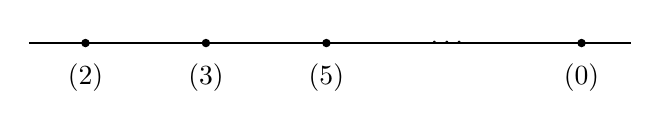
\begin{tikzpicture}[scale=0.9]
  \draw[thick] (-0.8,0) -- (7.7,0);
  \fill (0,0) circle (1.7pt) node[below=4pt] {$(2)$};
  \fill (1.7,0) circle (1.7pt) node[below=4pt] {$(3)$};
  \fill (3.4,0) circle (1.7pt) node[below=4pt] {$(5)$};
  \node at (5.1,0) {$\cdots$};
  \fill (7.0,0) circle (1.7pt) node[below=4pt] {$(0)$};
\end{tikzpicture}
\caption{$\Spec\mathbb{Z}$ 的「一幅图」，看起来与图~\ref{fig:a1c-picture} 可疑地相像。（依原书手绘图重绘。）}\label{fig:spec-z-picture}
\end{figure}

让我们毫无愧色地把关于函数的那套讨论照搬到这个空间上。$100$ 是 $\Spec\mathbb{Z}$ 上的一个函数。它在 $(3)$ 处的值是「$1\pmod{3}$」；它在 $(2)$ 处的值是「$0\pmod{2}$」，而且实际上是一个二重零点。$\frac{27}{4}$ 是 $\Spec\mathbb{Z}$ 上的一个「\trRationalFunction」，在 $(2)$ 之外处处有定义。我们想说：它在 $(2)$ 处有一个二重\trPole，在 $(3)$ 处有一个三重零点。它在 $(5)$ 处的值为
\[
27\times 4^{-1}\equiv 2\times(-1)\equiv 3\pmod{5}.
\]
（我们会随着时间的推移逐步把这段讨论精确化。）

\textbf{例~4（幼稚但重要的例子，外加德语里的「培根」一词）：}\footnote{译注：这个标题在玩谐音梗——德语 \emph{Speck} 意为「培根」，读音正似 $\Spec k$（「speck」）。}$k$ 为任一\trField{}时，集合 $\Spec k$ 无聊得很：一个点。$\Spec 0$（其中 $0$ 是\trZeroRing）则是空集，因为 $0$ 没有\trPrimeIdeal。

\begin{exercise}[关于小概形的小练习]\label{ex:small-schemes-dual-numbers}
(a)~描述集合 $\Spec k[\epsilon]/(\epsilon^2)$。环 $k[\epsilon]/(\epsilon^2)$ 称为\textbf{\trDualNumbers{}环}（ring of dual numbers），日后会显得相当有用。你应当把 $\epsilon$ 想成一个非常小的数，小到它的平方是 $0$（虽然它本身不是 $0$）。它是一个非零函数，却在所有点上都取值为零——这给了我们的第一个「函数并不由其在各点处的值决定」的例子。我们将在 \S3.2.12 中进一步讨论这个现象。

(b)~描述集合 $\Spec k[x]_{(x)}$（关于\trLocalization{}的讨论见 \S1.2.3）。从 \S3.2.9 与练习~3.4.K 开始，我们会反复遇见这个概形。日后你或许会把它看作一条相当好的「光滑曲线」的一片碎片。
\end{exercise}

在例~2 中我们把情形限制在\trAlgClosedField，这是有原因的：若域不是代数闭的，事情会更加微妙。

\textbf{例~5（$\mathbb{R}$ 上的\trAffineLine）：}$\mathbb{A}^1_{\mathbb{R}}=\Spec\mathbb{R}[x]$。利用 $\mathbb{R}[x]$ 是\textbf{\trEuclideanDomain}（Euclidean domain）这一事实，与例~1--3 类似的论证表明：其\trPrimeIdeal{}为 $(0)$、$(x-a)$（$a\in\mathbb{R}$），以及 $(x^2+ax+b)$（其中 $x^2+ax+b$ 是\trIrreducible{}的二次式）。后两类都是\trMaximalIdeal，也就是说，对它们取商皆得\trField。例如：$\mathbb{R}[x]/(x-3)\cong\mathbb{R}$，$\mathbb{R}[x]/(x^2+1)\cong\mathbb{C}$。

\begin{exercise}[不重要练习]\label{ex:irreducible-quadratic-quotient-c}
证明：对最后一类形如 $(x^2+ax+b)$ 的素理想，其商总同构于 $\mathbb{C}$。
\end{exercise}

这样我们就有了实直线上本来就会指望见到的那些点，它们对应实数；有\trGenericPoint{} $0$；还有新的点，我们可以把它们解释为复数的\emph{\trConjugate{}对}（conjugate pairs）（即那个二次式的根）。这最后一类点应当被看作与实数、而非与\trGenericPoint{}更亲近。你可以把 $\mathbb{A}^1_{\mathbb{R}}$ 想象成沿实轴对折起来的复平面。但关键在于：\trGalois{}\trConjugate{}的点（比如 $i$ 与 $-i$）被视为粘在一起。

我们来探索这个空间上的函数。考虑函数 $f(x)=x^3-1$。它在点 $[(x-2)]$ 处的值是 $7$，或者说得更妥帖些，「$7\pmod{x-2}$」。那么在 $(x^2+1)$ 处呢？我们得到
\[
x^3-1\equiv -x-1\pmod{x^2+1},
\]
而这可以卓有成效地解释为 $-i-1$。

本例的一个寓意是：只要愿意，我们可以在非代数闭的域上工作。这固然更复杂，但我们所关心的信息大半仍能找回。

\begin{exercise}[重要练习]\label{ex:affine-line-over-q}
描述集合 $\mathbb{A}^1_{\mathbb{Q}}$。（要画出类似 $\mathbb{A}^1_{\mathbb{R}}$ 那样的图更难。但如图~\ref{fig:a1c-picture} 那样「在一条直线上撒点」的粗略漫画，仍不失为一幅合理的草图。）
\end{exercise}

\textbf{例~6（$\mathbb{F}_p$ 上的\trAffineLine）：}$\mathbb{A}^1_{\mathbb{F}_p}=\Spec\mathbb{F}_p[x]$。与前几例一样，$\mathbb{F}_p[x]$ 是\trEuclideanDomain，故其\trPrimeIdeal{}形如 $(0)$ 或 $(f(x))$，其中 $f(x)\in\mathbb{F}_p[x]$ 是一个次数任意的\trIrreducible{}多项式。\trIrreducible{}多项式对应于 $\mathbb{F}_p$ 上的若干\trGalois{}\trConjugate{}点集。

注意，$\Spec\mathbb{F}_p[x]$ 有 $p$ 个点对应于 $\mathbb{F}_p$ 的元素，但还有多得多的点（无穷多，见\cref{ex:spec-kx-infinite}）。这使得这个空间远比「$p$ 个点」丰富。例如，多项式 $f(x)$ 并不由其在 $\mathbb{F}_p$ 的 $p$ 个元素上的值决定，但它\emph{确实}由其在 $\Spec\mathbb{F}_p[x]$ 的各点处的值决定。（如我们先前所说，这并非对所有概形成立。）

即便你是搞几何的人，也应当琢磨琢磨这件事——这种直觉日后会在几何情形中再现。哪怕你自以为只对在\trAlgClosedField{}（比如 $\mathbb{C}$）上工作感兴趣，也终会被迫面对非代数闭的域（比如 $\mathbb{C}(x)$）。

\begin{exercise}\label{ex:spec-kx-infinite}
若 $k$ 是\trField，证明 $\Spec k[x]$ 有无穷多个点。（提示：\trn{Euclid}{欧几里得}关于 $\mathbb{Z}$ 的素数无穷的证明。）
\end{exercise}

\textbf{例~7（复仿射平面）：}$\mathbb{A}^2_{\mathbb{C}}=\Spec\mathbb{C}[x,y]$。（与例~1、例~2 一样，把 $\mathbb{C}$ 换成\emph{任何}\trAlgClosedField，我们的讨论照样适用。）可惜，$\mathbb{C}[x,y]$ 不是\trPID：$(x,y)$ 不是一个主理想。我们可以很快叫出\emph{一些}\trPrimeIdeal{}的名字。其一是 $(0)$，它同前几例中的诸 $(0)$ 味道相仿。$(x-2,\,y-3)$ 是素的，而且甚至是极大的，因为 $\mathbb{C}[x,y]/(x-2,\,y-3)\cong\mathbb{C}$，这个同构由 $f(x,y)\mapsto f(2,3)$ 给出。更一般地，对任意 $(a,b)\in\mathbb{C}^2$，$(x-a,\,y-b)$ 都是素的。此外，若 $f(x,y)$ 是\trIrreducible{}多项式（例如 $y-x^2$ 或 $y^2-x^3$），则 $(f(x,y))$ 是素的。

\begin{exercise}\label{ex:prime-ideals-cxy}
证明我们已经找全了 $\mathbb{C}[x,y]$ 的\trPrimeIdeal。提示：设 $\mathfrak{p}$ 是一个非主的\trPrimeIdeal。证明可以找到无公因子的 $f(x,y)$ 与 $g(x,y)$，二者都含于 $\mathfrak{p}$。考虑\trEuclideanDomain{} $\mathbb{C}(x)[y]$ 中的欧几里得算法，证明可以找到非零的 $h(x)\in(f(x,y),\,g(x,y))\subset\mathfrak{p}$。利用素性，证明 $h(x)$ 的某个线性因子（比如说 $(x-a)$）位于 $\mathfrak{p}$ 中。同理证明存在某个 $(y-b)\in\mathfrak{p}$。
\end{exercise}

\begin{figure}[htbp]
\centering
\begin{tikzpicture}[scale=1.0]
  \draw[gray!60,thick,->] (-2.8,0) -- (3.0,0);
  \draw[gray!60,thick,->] (0,-2.3) -- (0,2.5);
  \draw[thick] (-1.9,2.3) .. controls (-1.0,1.2) and (-0.5,0.5) .. (0.3,0.55)
    .. controls (1.0,0.6) and (1.05,1.5) .. (0.45,1.62)
    .. controls (-0.05,1.72) and (-0.4,1.15) .. (0.15,0.85)
    .. controls (0.8,0.55) and (1.6,-0.4) .. (2.45,-1.3);
  \fill (-1.7,-0.6) circle (1.9pt);
  \node[anchor=north east,align=right] at (-1.55,-0.72)
    {$(a,b)=[(x-a,\,y-b)]$\\「闭点」（见定义~3.6.8）};
  \node at (1.15,1.35) {$\cdots$};
  \fill (1.6,1.5) circle (1.9pt);
  \node[anchor=west] at (1.72,1.1) {$[(f(x,y))]$};
  \node[anchor=east] at (1.55,-1.55) {$[(0)]$};
  \fill (1.82,-1.45) circle (0.55pt);
  \fill (1.98,-1.25) circle (0.95pt);
  \fill (2.2,-0.95) circle (1.5pt);
\end{tikzpicture}
\caption{画出 $\mathbb{A}^2_{\mathbb{C}}=\Spec\mathbb{C}[x,y]$。（依原书手绘图重绘。）}\label{fig:a2c-picture}
\end{figure}

现在我们试着画出 $\mathbb{A}^2_{\mathbb{C}}$ 的图（见图~\ref{fig:a2c-picture}）。$\mathbb{C}[x,y]$ 的极大素理想对应于 $\mathbb{C}^2$ 中的传统点：$[(x-a,\,y-b)]$ 对应于 $(a,b)\in\mathbb{C}^2$。现在我们得把「附赠点」也想象出来。$[(0)]$ 不知怎地栖身于所有传统点的背后；它在仿射平面的某处，却又不在任何特定的地方。例如，它并不落在抛物线 $y=x^2$ 上。点 $[(y-x^2)]$ 落在抛物线 $y=x^2$ 上，却又不在抛物线的任何特定位置上。（图~\ref{fig:a2c-picture} 有点误导。比如，点 $[(0)]$ 并不在第四象限；它不知怎地邻近其他每一个点，这就是为什么图中把它画成一个略微发散的大点。）从这幅图你能看出，我们其实已经在暗地里思考「维数」了。\trPrimeIdeal{} $(x-a,\,y-b)$ 不知怎地是 $0$ 维的，\trPrimeIdeal{} $(f(x,y))$ 是 $1$ 维的，而 $(0)$ 是 $2$ 维的。（我们在这里谈的维数全是\emph{复}维数或\emph{代数}维数。复平面 $\mathbb{C}^2$ 的实维数是 $4$，复维数是 $2$。复维数一般是实维数的一半。）要到第 12 章我们才会精确定义\trDimension，但在那之前你尽管把它记在心上。

还要注意：\trMaximalIdeal{}对应于「最小」的点。更小的理想对应「更大」的点。「一个\trPrimeIdeal{}包含另一个」说的是那些点「具有相反的包含关系」。等我们有了\trTopology，这一切都会变得精确。这种序的反转有点令人困惑，而且即便在概念精确化之后也仍会如此。

现在我们来看例~7 的显然推广。

\textbf{例~8（复仿射 $n$ 空间——重要！）：}令 $\mathbb{A}^n_{\mathbb{C}}:=\Spec\mathbb{C}[x_1,\dots,x_n]$。（重要定义：更一般地，$\mathbb{A}^n_A$ 定义为 $\Spec A[x_1,\dots,x_n]$，其中 $A$ 是任意\trRing。当基环在上下文中清楚时，下标 $A$ 常被省去。给学究的一句：记号 $\mathbb{A}^n_A$ 隐含地包括了 $n$ 个\textbf{\trCoordinate{}函数}（coordinate functions）$x_1,\dots,x_n$ 这份数据。）为具体起见，取 $n=3$。于是一个起初看似纯代数的问题变得有趣起来：$\mathbb{C}[x,y,z]$ 的\trPrimeIdeal{}是什么？

与之前类似，$(x-a,\,y-b,\,z-c)$ 是一个\trPrimeIdeal。它是\trMaximalIdeal，因为其\trResidueRing{}（residue ring）是一个\trField{}（即 $\mathbb{C}$）；我们把这些点看作「零维点」。基于对这些理想的几何解释，我们将经常把 $[(x-a,\,y-b,\,z-c)]$ 写作 $(a,b,c)$。不会再有别的\trMaximalIdeal{}了，依据是\trHilbert{}弱\trNullstellensatz（\cref{thm:hilbert-weak-nullstellensatz}）。

\vkthmsync{5}
\begin{theorem}[\trHilbert{}弱\trNullstellensatz]\label{thm:hilbert-weak-nullstellensatz}
若 $k$ 是\trAlgClosedField，则 $k[x_1,\dots,x_n]$ 的\trMaximalIdeal{}恰是形如 $(x_1-a_1,\dots,x_n-a_n)$（其中 $a_i\in k$）的那些\trIdeal。
\end{theorem}

我们不妨顺手把一个略强的版本也在此陈述了。

\begin{theorem}[\trHilbert{}\trNullstellensatz]\label{thm:hilbert-nullstellensatz}
若 $k$ 是任意\trField，则 $k[x_1,\dots,x_n]$ 的每个\trMaximalIdeal{}的\trResidueField{}都是 $k$ 的\trFiniteFieldExtension。翻译一下：任何域扩张，只要作为 $k$-代数是有限生成的，就必然作为 $k$-向量空间也是有限生成的（即它是域的\trFiniteFieldExtension）。
\end{theorem}

这条陈述也常被称作\trZariski{}引理。

\begin{exercise}\label{ex:hilbert-nullstellensatz-implies-weak}
证明\trNullstellensatz（\cref{thm:hilbert-nullstellensatz}）蕴含弱\trNullstellensatz（\cref{thm:hilbert-weak-nullstellensatz}）。
\end{exercise}

我们将在 \S8.4.3 证明\trNullstellensatz，并在练习~12.2.B 中再证一次。

下面这个事实是\trNullstellensatz{}的有用搭档。

\begin{exercise}[无须\trNullstellensatz]\label{ex:finite-algebra-domain-field}
任何是有限 $k$-代数的\trIntegralDomain{} $A$（即作为 $k$-向量空间有限维的 $k$-代数）必是\trField。提示：对任意非零 $x\in A$，证明 $\times x\colon A\to A$ 是\trIsomorphism。（于是，与\cref{thm:hilbert-nullstellensatz}相结合便知：\emph{具有有限维剩余环的 $k[x_1,\dots,x_n]$ 的\trPrimeIdeal，恰同于 $k[x_1,\dots,x_n]$ 的\trMaximalIdeal。}这一点值得记住。）
\end{exercise}

$\mathbb{C}[x,y,z]$ 还有别的\trPrimeIdeal。我们有 $(0)$，它对应一个「三维点」。我们有 $(f(x,y,z))$，其中 $f$ \trIrreducible；与之相联系的是「\trHypersurface」（hypersurface）$f=0$，所以这一类在本性上是「二维」的。但我们并没有找全它们！一条线索：我们有了「维数」$0$、$2$、$3$ 的\trPrimeIdeal——还缺「维数 $1$」。这样的一个\trPrimeIdeal{}便是 $(x,y)$。我们把它描绘成 $x=y=0$ 的\trLocus，即 $z$-轴。它是一个\trPrimeIdeal，因为相应的商 $\mathbb{C}[x,y,z]/(x,y)\cong\mathbb{C}[z]$ 是\trIntegralDomain（而且应当被解释为 $z$-轴上的函数）。「一维素理想」有很多，而且没有办法以合理的方式将它们分类。日后会看到，它们对应于我们视为\trIrreducible{}曲线的东西。于是，这个纯代数问题（「$\mathbb{C}[x,y,z]$ 的\trPrimeIdeal{}是什么」）的答案竟然在根本上是几何的！

$\mathbb{A}^1_{\mathbb{Q}}$ 中对应于环 $\mathbb{Q}[x]$ 的\trMaximalIdeal{}的那些点（我们很快会称之为「\trClosedPoint」；见定义~3.6.8）可以解释为 $\overline{\mathbb{Q}}$ 中把\trGalois{}共轭点粘合起来的点（\cref{ex:affine-line-over-q}）；这一事实可推广到 $\mathbb{A}^n_{\mathbb{Q}}$。例如在 $\mathbb{A}^2_{\mathbb{Q}}$ 中，$(\sqrt{2},\sqrt{2})$ 与 $(-\sqrt{2},-\sqrt{2})$ 粘在一起，但与 $(\sqrt{2},-\sqrt{2})$ 不粘。下面的练习会让你略微体会这是怎么回事。

\begin{exercise}\label{ex:maximal-ideals-sqrt2}
描述 $\mathbb{Q}[x,y]$ 中对应于 $(\sqrt{2},\sqrt{2})$ 与 $(-\sqrt{2},-\sqrt{2})$ 的\trMaximalIdeal。再描述 $\mathbb{Q}[x,y]$ 中对应于 $(\sqrt{2},-\sqrt{2})$ 与 $(-\sqrt{2},\sqrt{2})$ 的\trMaximalIdeal。两种情形下的\trResidueField{}各是什么？
\end{exercise}

$\mathbb{A}^2_{\mathbb{Q}}$ 的「\trClosedPoint」（即对应于环 $\mathbb{Q}[x,y]$ 的\trMaximalIdeal{}的那些点）可以描述为 $\overline{\mathbb{Q}}^2$ 中各点的\trGalois{}轨道；这套描述甚至可以推广到其他「非闭」点上，如下。

\begin{exercise}[不重要但棘手而有趣的练习]\label{ex:map-c2-a2q}
考虑集合的映射 $\phi\colon\mathbb{C}^2\to\mathbb{A}^2_{\mathbb{Q}}$，定义如下：$(z_1,z_2)$ 被送到 $\mathbb{Q}[x,y]$ 中由在 $(z_1,z_2)$ 处消失的多项式所组成的\trPrimeIdeal。

(a)~$(\pi,\pi^2)$ 的像是什么？

(b)~\hard\ 证明 $\phi$ 是满射。（警示：你需要一些我们还没讨论过的想法才能解决它。等我们在 $\mathbb{A}^2_{\mathbb{Q}}$ 上定义了\trZariskiTopology，你将能验证 $\phi$ 是\trContinuousMap，其中 $\mathbb{C}^2$ 带的是\trClassicalTopology。这个例子可以推广。比如，日后你也许能把它推广到任意维数。）
\end{exercise}

\textbf{3.2.7.\ 商与局部化。}\quad 从旧环得到新环的两条自然途径——取商与取局部化——在谱的语言中有其解读。

\textbf{3.2.8.\ 商：$\Spec A/I$ 作为 $\Spec A$ 的子集。}\quad 一个重要的事实是：$A/I$ 的\trPrimeIdeal{}与 $A$ 的包含 $I$ 的\trPrimeIdeal{}成双射。

\begin{exercise}[必做代数练习：此前从未见过则必做]\label{ex:quotient-primes-bijection}
设 $A$ 是\trRing，$I$ 是 $A$ 的一个\trIdeal。令 $\phi\colon A\to A/I$。证明 $\phi^{-1}$ 给出 $A/I$ 的\trPrimeIdeal{}与 $A$ 的包含 $I$ 的\trPrimeIdeal{}之间保持包含关系的双射。于是我们可以把 $\Spec A/I$ 描画为 $\Spec A$ 的一个子集。
\end{exercise}

作为一个重要的动机性特例，你如今便有了\emph{仿射复簇}（affine complex varieties）的一幅图景。设 $A$ 是有限生成的 $\mathbb{C}$-代数，由 $x_1,\dots,x_n$ 生成，带关系 $f_1(x_1,\dots,x_n)=\cdots=f_r(x_1,\dots,x_n)=0$。那么这套「生成元与关系」的描述自然让我们能把 $\Spec A$ 解释为 $\mathbb{A}^n_{\mathbb{C}}$ 的一个子集——我们把它想成「传统点」（复数的 $n$ 元组）连同一些我们尚未完全描述的「附赠点」。要看哪些传统点落在 $\Spec A$ 里，只需解方程 $f_1=\cdots=f_r=0$。例如，$\Spec\mathbb{C}[x,y,z]/(x^2+y^2-z^2)$ 可以画作图~\ref{fig:cone-picture} 的模样。（诚然这只是「$\mathbb{R}$-点的草图」，但日后我们仍会觉得它有用。）整幅图景（连同\trNullstellensatz{}一起）在把 $\mathbb{C}$ 换成任何\trAlgClosedField{}后照搬无误。的确，对大多数\trAlgClosedField{} $k$，图~\ref{fig:cone-picture} 也可以说画的是 $\Spec k[x,y,z]/(x^2+y^2-z^2)$（尽管在特征 $2$ 时它有误导性，因为碰巧有 $x^2+y^2-z^2=(x+y+z)^2$）。

\begin{figure}[htbp]
\centering
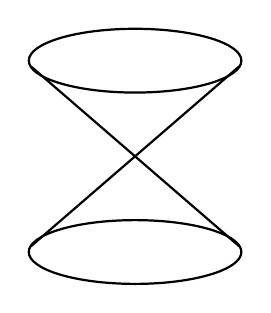
\begin{tikzpicture}[scale=0.9]
  \draw[thick] (0,1.35) ellipse (1.5 and 0.45);
  \draw[thick] (0,-1.35) ellipse (1.5 and 0.45);
  \draw[thick] (-1.47,1.27) -- (1.47,-1.27);
  \draw[thick] (1.47,1.27) -- (-1.47,-1.27);
\end{tikzpicture}
\caption{$\Spec\mathbb{C}[x,y,z]/(x^2+y^2-z^2)$ 的「一幅图」。（依原书手绘图重绘。）}\label{fig:cone-picture}
\end{figure}

\textbf{3.2.9.\ 局部化：$\Spec S^{-1}A$ 作为 $\Spec A$ 的子集。}\quad 下面的练习展示\trPrimeIdeal{}在局部化下的行为。

\begin{exercise}[必做代数练习：此前从未见过则必做]\label{ex:localization-primes-bijection}
设 $S$ 是 $A$ 的\trMultiplicativeSubset。描述 $S^{-1}A$ 的\trPrimeIdeal{}与 $A$ 中\emph{不与}\trMultiplicativeSubset{} $S$ 相交的\trPrimeIdeal{}之间保持序的双射。
\end{exercise}

回忆 \S1.2.3：局部化有两种重要的风味。第一种是 $A_f=\{1,f,f^2,\dots\}^{-1}A$，其中 $f\in A$；一个动机性的例子是 $A=\mathbb{C}[x,y]$、$f=y-x^2$。第二种是 $A_{\mathfrak{p}}=(A\smallsetminus\mathfrak{p})^{-1}A$，其中 $\mathfrak{p}$ 是\trPrimeIdeal；动机性的例子：$A=\mathbb{C}[x,y]$、$S=A\smallsetminus(x,y)$。

若 $S=\{1,f,f^2,\dots\}$，则 $S^{-1}A$ 的\trPrimeIdeal{}恰是那些不包含 $f$ 的\trPrimeIdeal——也就是「$f$ 不消失」的那些点。（在 \S3.5 中，等我们知道了\trOpenSet{}是什么，就会把这样的东西称作\emph{\trDistinguishedOpen}（distinguished open set）。）于是要画出 $\Spec\mathbb{C}[x,y]_{y-x^2}$，就先画仿射平面，然后扔掉抛物线 $y-x^2=0$ 上的那些点——即诸点 $(a,a^2)$（$a\in\mathbb{C}$）（意思是 $[(x-a,\,y-a^2)]$），以及「新一类的点」$[(y-x^2)]$。

思考「倒转\trZerodivisor」情形下的局部化，起初可能令人困惑，因为此时局部化 $A\to S^{-1}A$ 不是\trInjectiveMap（\cref{ex:when-localization-is-injective}）。几何直观能帮上忙。考虑 $A=\mathbb{C}[x,y]/(xy)$、$f=x$ 的情形。局部化 $A_f$ 是什么？空间 $\Spec\mathbb{C}[x,y]/(xy)$「就是」仿射平面中两条坐标轴之并。局部化意味着扔掉 $x$ 消失的\trLocus。于是剩下的就是 $x$-轴挖去原点，因此我们预期得到 $\Spec\mathbb{C}[x]_x$。所以应当有某个自然的\trIsomorphism
\[
(\mathbb{C}[x,y]/(xy))_x\stackrel{\ \sim\ }{\longrightarrow}\mathbb{C}[x]_x.
\]

\begin{exercise}\label{ex:xy-localization-isomorphism}
证明这两个环同构。（你将看到，左边的 $y$ 到了右边变成 $0$。）
\end{exercise}

若 $S=A\smallsetminus\mathfrak{p}$，则 $S^{-1}A$ 的\trPrimeIdeal{}恰是 $A$ 的含于 $\mathfrak{p}$ 的那些\trPrimeIdeal。在我们的例子 $A=\mathbb{C}[x,y]$、$\mathfrak{p}=(x,y)$ 中，我们保留所有对应于「穿过原点的东西」的点，即零维点 $(x,y)$、二维点 $(0)$，以及满足 $f(0,0)=0$ 的一维点 $(f(x,y))$，也就是那些「穿过原点的\trIrreducible{}曲线」。你可以把这想象成原点近旁平面的一片碎片；凡在原点处实际上「看不见」的东西都被丢弃（见图~\ref{fig:shred-of-a2}）。

\begin{figure}[htbp]
\centering
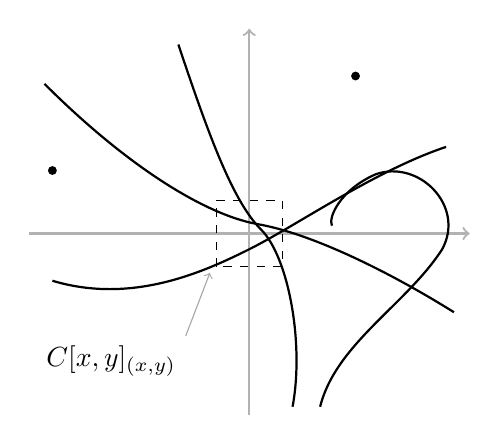
\begin{tikzpicture}[scale=1.0]
  \draw[gray!60,thick,->] (-2.8,0) -- (2.8,0);
  \draw[gray!60,thick,->] (0,-2.3) -- (0,2.6);
  \draw[thick] (-0.9,2.4) .. controls (-0.5,1.2) and (-0.2,0.4) .. (0.15,0.05)
    .. controls (0.5,-0.3) and (0.7,-1.4) .. (0.55,-2.2);
  \draw[thick] (-2.6,1.9) .. controls (-1.6,0.9) and (-0.6,0.25) .. (0.1,0.12)
    .. controls (0.8,0.0) and (1.8,-0.5) .. (2.6,-1.0);
  \draw[thick] (-2.5,-0.6) .. controls (-1.5,-0.9) and (-0.6,-0.5) .. (0.0,-0.2)
    .. controls (0.6,0.1) and (1.6,0.8) .. (2.5,1.1);
  \draw[thick] (0.9,-2.2) .. controls (1.1,-1.4) and (2.0,-0.9) .. (2.45,-0.2)
    .. controls (2.75,0.35) and (2.15,0.95) .. (1.6,0.75)
    .. controls (1.15,0.55) and (1.0,0.2) .. (1.05,0.1);
  \draw[dashed] (-0.42,-0.42) rectangle (0.42,0.42);
  \fill (1.35,2.0) circle (1.6pt);
  \fill (-2.5,0.8) circle (1.6pt);
  \node[anchor=north west] (speclab) at (-2.7,-1.3) {$\Spec \mathbb{C}[x,y]_{(x,y)}$};
  \draw[gray!70,->] (speclab.north east) -- (-0.5,-0.5);
\end{tikzpicture}
\caption{把 $\Spec \mathbb{C}[x,y]_{(x,y)}$ 画作「$\mathbb{A}^2_{\mathbb{C}}$ 的一片碎片」：只剩下原点附近的那些点。（依原书手绘图重绘。）}\label{fig:shred-of-a2}
\end{figure}

另一个例子：$A=k[x]$、$\mathfrak{p}=(x)$（或者更一般地，$\mathfrak{p}$ 是任一\trMaximalIdeal）。此时 $A_{\mathfrak{p}}$ 只有两个\trPrimeIdeal（\cref{ex:small-schemes-dual-numbers}(b)）。你应当把它看作一条「光滑曲线」的\trGerm：其中一个点是「经典点」，另一个点则是「曲线的\trGenericPoint」。这是\trDVR{}（discrete valuation ring）的一个例子；而事实上，一切\trDVR{}都应当这样来直观化。我们将在 \S13.5 讨论\trDVR。到那时，「光滑」与「曲线」这两个词的用法都将得到辩护。（现实检验：试着把 $\mathbb{Z}$ 在 $(2)$ 处与在 $(0)$ 处的局部化的谱画出来。这两幅图有何不同？）

\textbf{3.2.10.\ 重要事实：环的映射诱导谱的映射（作为集合）。}\quad 我们现在做一条观察，它日后将成长为概形态射的概念。

\begin{exercise}[重要而容易的练习]\label{ex:preimage-of-prime-ideal}
若 $\phi\colon B\to A$ 是环映射，而 $\mathfrak{p}$ 是 $A$ 的一个\trPrimeIdeal，证明 $\phi^{-1}(\mathfrak{p})$ 是 $B$ 的\trPrimeIdeal。
\end{exercise}

于是，环映射 $\phi\colon B\to A$ 诱导一个「方向相反」的集合映射 $\Spec A\to\Spec B$。这给出一个从\trRing{}的\trCategory{}到\trSet{}的\trCategory{}的\trContravariantFunctor：两个环映射的复合诱导相应的谱映射的复合。

\begin{exercise}[容易的练习：现实检验]\label{ex:inclusion-quotient-localization}
设 $B$ 是\trRing。
(a)~设 $I\subset B$ 是一个\trIdeal。证明映射 $\Spec B/I\to\Spec B$ 就是 \S3.2.8 的那个包含。
(b)~设 $S\subset B$ 是乘性子集。证明映射 $\Spec S^{-1}B\to\Spec B$ 就是 \S3.2.9 的那个包含。
\end{exercise}

\textbf{3.2.11.\ 一个显式的例子。}\quad 在「仿射复簇」（或者确实，任何\trAlgClosedField{}上的仿射簇）的情形，由显式公式给出的映射与环映射之间的翻译相当直接。例如，考虑从 $\mathbb{C}^2$ 中由 $b=a^2$ 给出的抛物线（\trCoordinate{}为 $a$ 与 $b$）到 $\mathbb{C}^3$ 中由方程 $y=x^2$ 与 $z=y^2$ 割出的「曲线」（\trCoordinate{}为 $x$、$y$、$z$）的一个映射。设该映射把点 $(a,b)\in\mathbb{C}^2$ 送到点 $(a,b,b^2)\in\mathbb{C}^3$。在我们的新语言中，我们有一个映射
\[
\Spec \mathbb{C}[a,b]/(b-a^2)\longrightarrow \Spec \mathbb{C}[x,y,z]/(y-x^2,\ z-y^2)
\]
由下式给出：
\[
\mathbb{C}[a,b]/(b-a^2)\longleftarrow\mathbb{C}[x,y,z]/(y-x^2,\ z-y^2),
\]
\[
(a,b,b^2)\longmapsto(x,y,z),
\]
即 $x\mapsto a$、$y\mapsto b$、$z\mapsto b^2$。如果这个想法还不清楚，下面两道练习非常值得做——头一次见到时它们可能极其令人困惑，而等你终于想通之时，它们又极具启发性（而且是平凡的）。

\begin{figure}[htbp]
\centering
\begin{tikzpicture}[scale=0.9]
  \draw[very thick] (-2.6,-1.7) -- (-2.6,2.4);
  \node at (-2.6,-2.2) {$y$-线};
  \draw[thick] plot[domain=-1.75:1.75,samples=41] ({\x+1.5},{\x*\x-1.6});
  \node at (1.5,-2.2) {$x$-线};
  \draw[gray!70,->] (0.3,0.75) -- (-1.9,0.75);
\end{tikzpicture}
\caption{由 $x\mapsto y=x^2$ 给出的映射 $\mathbb{C}\to\mathbb{C}$。（依原书手绘图重绘。）}\label{fig:parabola-map}
\end{figure}

\begin{exercise}[重要练习：特例]\label{ex:parabola-projection-special-case}
考虑复流形之间的映射 $\mathbb{C}\to\mathbb{C}$，由 $x\mapsto y=x^2$ 给出。我们把「源」$\mathbb{C}$ 解释为「$x$-线」，把「目标」$\mathbb{C}$ 解释为「$y$-线」。你可以把它想象为 $xy$-平面中的抛物线 $y=x^2$ 到 $y$-轴的投影（见图~\ref{fig:parabola-map}）。把相应的环映射解释为由 $y\mapsto x^2$ 给出的 $\mathbb{C}[y]\to\mathbb{C}[x]$。利用上文给出的定义（把 $a$ 与 $[(y-a)]$ 等同，把 $\sqrt{a}$ 与 $[(x-\sqrt{a})]$ 等同），验证点 $a\in\mathbb{C}$ 上方的原像（即\trFiber）是点（们）$\pm\sqrt{a}\in\mathbb{C}$。（本例的一个更成熟的版本出现在例~10.3.4 中。警示：在那里的 $x$ 与 $y$ 角色互换，为的是以某种方式描绘二重覆盖。）
\end{exercise}

\begin{exercise}[重要练习：推广例~3.2.11]\label{ex:polynomial-map-of-spectra}
设 $k$ 是\trField，并给定 $f_1,\dots,f_n\in k[x_1,\dots,x_m]$。令 $\phi\colon k[y_1,\dots,y_n]\to k[x_1,\dots,x_m]$ 是由 $y_i\mapsto f_i$ 定义的 $k$-代数之间的\trMorphism。
(a)~证明：对任意满足 $\phi(J)\subset I$ 的\trIdeal{} $I\subset k[x_1,\dots,x_m]$ 与 $J\subset k[y_1,\dots,y_n]$，$\phi$ 诱导集合的映射 $\Spec k[x_1,\dots,x_m]/I\to\Spec k[y_1,\dots,y_n]/J$。（你不妨先考虑 $I=0$、$J=0$ 的情形。事实上，(a) 与 $k$-代数毫无关系；你也可以在把环 $k[x_1,\dots,x_m]$ 与 $k[y_1,\dots,y_n]$ 换成一般的\trRing{} $A$ 与 $B$ 时证明这条陈述。）
(b)~证明 (a) 中的映射把点 $(a_1,\dots,a_m)\in k^m$（更精确地，$[(x_1-a_1,\dots,x_m-a_m)]\in\Spec k[x_1,\dots,x_m]$）送到
\[
(f_1(a_1,\dots,a_m),\ \dots,\ f_n(a_1,\dots,a_m))\in k^n.
\]
\end{exercise}

\begin{exercise}[练习：画出 $\mathbb{A}^n_{\mathbb{Z}}$]\label{ex:affine-space-over-z-picture}
考虑集合的映射 $\pi\colon\mathbb{A}^n_{\mathbb{Z}}\to\Spec\mathbb{Z}$，由环映射 $\mathbb{Z}\to\mathbb{Z}[x_1,\dots,x_n]$ 给出。若 $p$ 是素数，请描述纤维 $\pi^{-1}([(p)])$ 与 $\mathbb{A}^n_{\mathbb{F}_p}$ 之间的双射。（你无须描述这两个集合中的任何一个！这倒是好事，因为你根本办不到。）本练习也许会让你体味到该如何描绘映射（见图~\ref{fig:an-over-z-family}），尤其是为什么你可以把 $\mathbb{A}^n_{\mathbb{Z}}$ 想成 $\Spec\mathbb{Z}$ 上的一个「$\mathbb{A}^n$-丛」。（你能把 $[(0)]$ 之上的纤维解释成某个域 $k$ 的 $\mathbb{A}^n_k$ 吗？）
\end{exercise}

\begin{figure}[htbp]
\centering
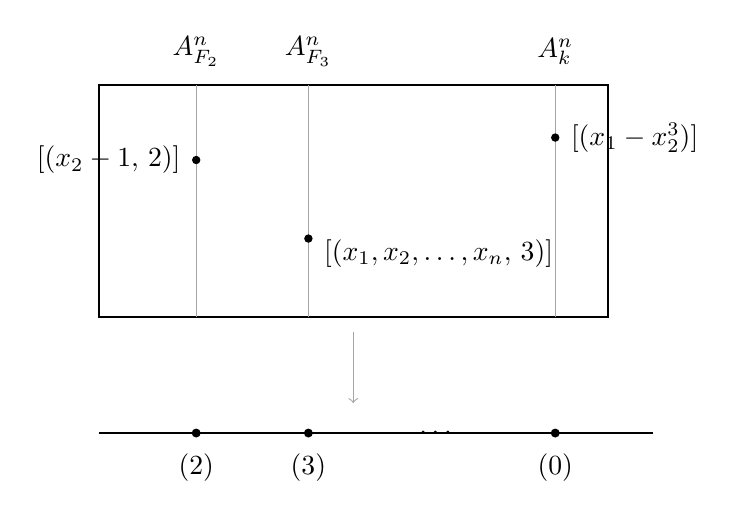
\begin{tikzpicture}[scale=0.95]
  \node at (0.4,2.65) {$\mathbb{A}^n_{\mathbb{F}_2}$};
  \node at (1.9,2.65) {$\mathbb{A}^n_{\mathbb{F}_3}$};
  \node at (5.2,2.65) {$\mathbb{A}^n_{k}$};
  \draw[thick] (-0.9,-0.9) rectangle (5.9,2.2);
  \draw[gray!70] (0.4,2.2) -- (0.4,-0.9);
  \draw[gray!70] (1.9,2.2) -- (1.9,-0.9);
  \draw[gray!70] (5.2,2.2) -- (5.2,-0.9);
  \fill (0.4,1.2) circle (1.6pt);
  \node[anchor=east] at (0.32,1.2) {$[(x_2-1,\,2)]$};
  \fill (1.9,0.15) circle (1.6pt);
  \node[anchor=west] at (1.98,-0.05) {$[(x_1,x_2,\dots,x_n,\,3)]$};
  \fill (5.2,1.5) circle (1.6pt);
  \node[anchor=west] at (5.28,1.5) {$[(x_1-x_2^3)]$};
  \draw[gray!70,->] (2.5,-1.1) -- (2.5,-2.05);
  \draw[thick] (-0.9,-2.45) -- (6.5,-2.45);
  \fill (0.4,-2.45) circle (1.7pt) node[below=4pt] {$(2)$};
  \fill (1.9,-2.45) circle (1.7pt) node[below=4pt] {$(3)$};
  \node at (3.6,-2.45) {$\cdots$};
  \fill (5.2,-2.45) circle (1.7pt) node[below=4pt] {$(0)$};
\end{tikzpicture}
\caption{$\mathbb{A}^n_{\mathbb{Z}}\to\Spec\mathbb{Z}$ 的一幅图：画成「$\mathbb{A}^n$ 之族」，或者说「$\Spec\mathbb{Z}$ 上的 $\mathbb{A}^n$-丛」。$k$ 是什么域？应当怎样「几何地」思考图中标出的三个点？（依原书手绘图重绘。）}\label{fig:an-over-z-family}
\end{figure}

\textbf{3.2.12.\ 函数并不由其在各点处的值决定：这是幂零元之过。}\quad 本节我们以描述一些古怪的行为作结。我们正在发展一套机器，它将让我们得以把几何直观带进代数。有一处十分十分要紧的地方，你的直觉在那里会是错的，所以你现在就该知道这件事，并相应地调整你的直觉。正如\trMumford{}（[Mu2, p.~12]）所指出的：「概形的这个侧面，在\trGrothendieck{}定义它们之时是最为惊世骇俗的。」

设我们有一个在所有点处都消失的函数（环元素）。那么它未必是零函数！这个问题的翻译是：全体\trPrimeIdeal{}的交是否必然恰好是 $0$？答案是否定的，对\trDualNumbers{}环 $k[\epsilon]/(\epsilon^2)$ 这个例子便是明证：$\epsilon\neq0$，但 $\epsilon^2=0$。（我们在\cref{ex:small-schemes-dual-numbers}(a) 中见过这个环。）任何某次幂为零的函数自然落在全体\trPrimeIdeal{}的交之中。

\begin{exercise}\label{ex:nilpotents-and-nilradical}
某次幂为 $0$ 的环元素称为\textbf{\trNilpotent{}元}（nilpotents）。
(a)~证明：若 $I$ 是由\trNilpotent{}元组成的\trIdeal，则 \cref{ex:quotient-primes-bijection} 中的包含 $\Spec B/I\to\Spec B$ 是双射。于是\trNilpotent{}元不影响底集合。（我们很快将在 \S3.4.7 中看到，它们也不影响\trTopology——差别将在\trStructureSheaf{}之中。）
(b)~证明\trRing{} $B$ 的全体\trNilpotent{}元构成一个\trIdeal。这个\trIdeal{}称为\textbf{\trNilradical}（nilradical），记作 $\mathfrak{N}=\mathfrak{N}(B)$。
\end{exercise}

于是\trNilradical{}含于全体\trPrimeIdeal{}的交之中。逆命题也真：

\vkthmsync{13}
\begin{theorem}\label{thm:nilradical-intersection-primes}
\trNilradical{} $\mathfrak{N}(A)$ 是 $A$ 的全部\trPrimeIdeal{}的交。几何地说：$\Spec A$ 上的一个函数在每一点处都消失，当且仅当它是\trNilpotent{}的。
\end{theorem}

\begin{exercise}\label{ex:nilradical-theorem-proof}
如果你不知道这条定理，那就去查一查，或者更好的是，亲自证它。（提示：利用「$A$ 的任何\trProperIdeal{}都含于某个\trMaximalIdeal」这一事实，而这需要\trZornsLemma。可能的进一步提示：设 $x\notin\mathfrak{N}(A)$。我们要证明存在不含 $x$ 的\trPrimeIdeal。证明 $A_x$ 不是\trZeroRing，办法是证明 $1\neq0$。）
\end{exercise}

\textbf{3.2.14.}\quad 特别地，尽管「函数并不由其在各点处的值决定」令人不安，但我们已经把这种直觉失灵的确切内容指了出来：两个函数在各点处取值相同，当且仅当它们相差一个\trNilpotent{}元。你应当从几何上思考这件事：一个函数在\trRing{}的谱的每一点处都消失，当且仅当它有一次幂为零。而如果没有非零\trNilpotent{}元——若 $\mathfrak{N}=(0)$——那么函数\emph{确实}由其在各点处的值决定。如果一个\trRing{}没有非零\trNilpotent{}元，我们就称它是\textbf{\trReduced}（reduced）的。

\begin{exercise}[有趣的不重要练习：不用 $\delta$ 与 $\epsilon$ 的求导——至少不用 $\delta$]\label{ex:derivatives-dual-numbers}
设有多项式 $f(x)\in k[x]$。我们改在 $k[x,\epsilon]/(\epsilon^2)$ 中工作。那么 $f(x+\epsilon)$ 是什么？（先做几个例子，再证明你观察到的模式。）这是一个暗示：\trNilpotent{}元将在定义微分信息（第 21 章）时十分重要。
\end{exercise}
